\chapter{Технологический раздел}

\section{Язык программирования}
В качестве языка программирований выбран язык высокого уровня JavaScript.

\section{Примеры кода}

\begin{lstlisting}[caption={Событийный принцип: поиск минимального размера буферной памяти}]
function findMinLengthQueue(a, b, lambda, finishTime, releaseOrder) {
  let si = new SourceOfInformation(a, b);
  let su = new ServiceUnitByPoisson(releaseOrder, lambda);

  let bmLength = 0;
  let flagRun = true;

  while (flagRun) {
    ++bmLength;

    try {
      runSimulation(si, su, bmLength, finishTime);
    } catch (err) {
      flagRun = !flagRun;
    } finally {
      flagRun = !flagRun;
    }
  }

  return bmLength;
}

function runSimulation(si, su, bmLength, finishTime) {
  
  let bm = new Memory(bmLength);

  let fel = [];
  
  let blocks = [si, su];

  initBlock(fel, blocks, finishTime);


  while (true) {
    let iMin = getNumberMin(fel);

    if (iMin == blocks.length) {
      break;
    }

    blocks[iMin].run(bm);
    fel[iMin] += blocks[iMin].getNextTime()
  }
}
\end{lstlisting}

\begin{lstlisting}[caption={Принцип dt: поиск минимального размера буферной памяти}]
function findMinLengthQueue(dt, a, b, lambda, finishTime, releaseOrder) {
  let bmLength = 0;
  let flagRun = true;

  while (flagRun) {
    ++bmLength;

    try {
      let si = new SourceOfInformation(a, b);
      let su = new ServiceUnitByPoisson(releaseOrder, lambda);

      let bm = new Memory(bmLength);

      let nowTime = 0;
      let blocks = [si, su];

      while (nowTime < finishTime) {
        blocks.forEach(block => {
          block.run(nowTime, bm);
        })

        nowTime += dt;
      }
    } catch (err) {
      flagRun = !flagRun;
    } finally {
      flagRun = !flagRun;
    }
  }

  return bmLength;
}
\end{lstlisting}

\section{Взаимодейсвтие с пользователем}

Взаимодейсвтие с пользователем осуществляется через html страницы, открытые в браузере.

\begin{figure}
  \centering
  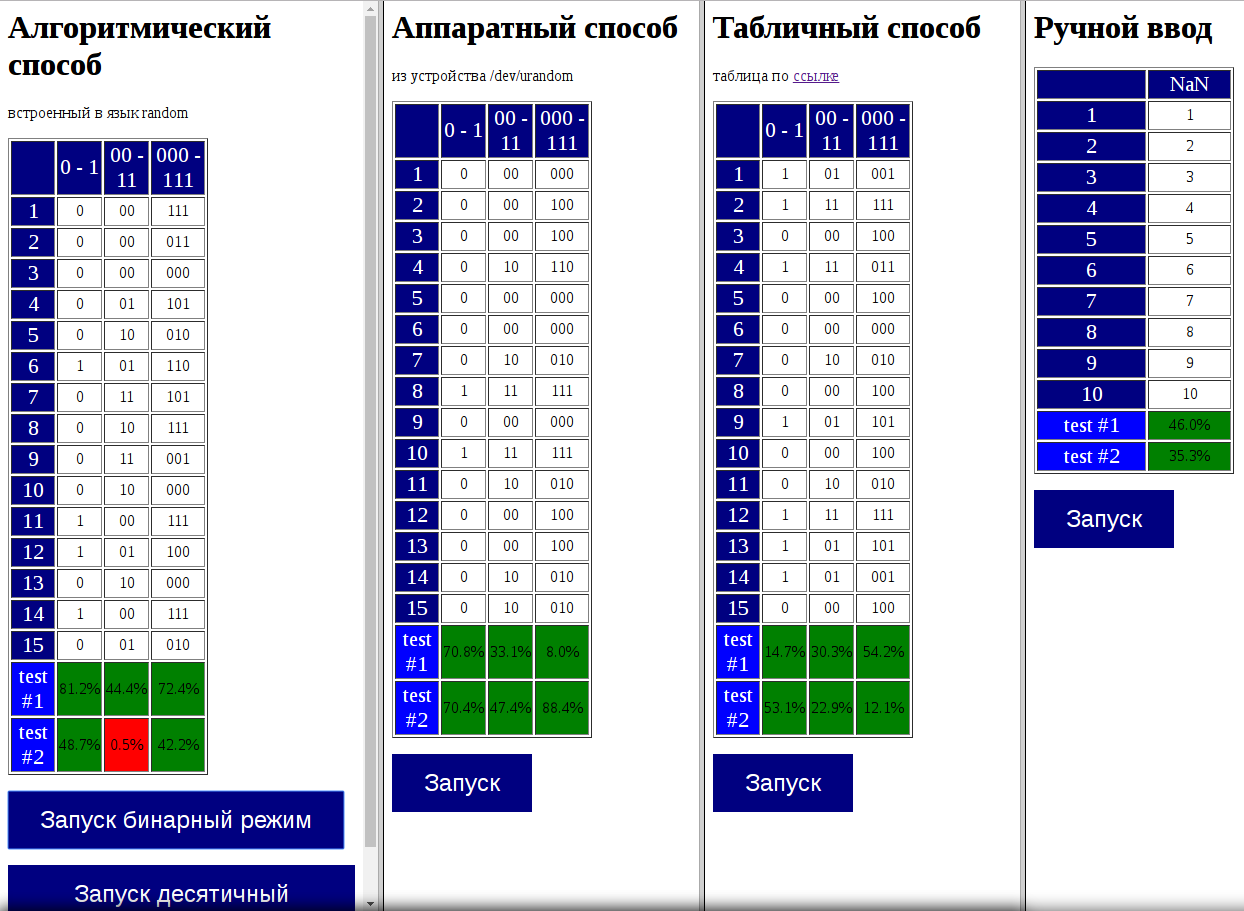
\includegraphics[scale=0.5]{screen1.png}
  \caption{Принцип $\Delta t$: поиск минимального размера буферной памяти}
\end{figure}

\begin{figure}
  \centering
  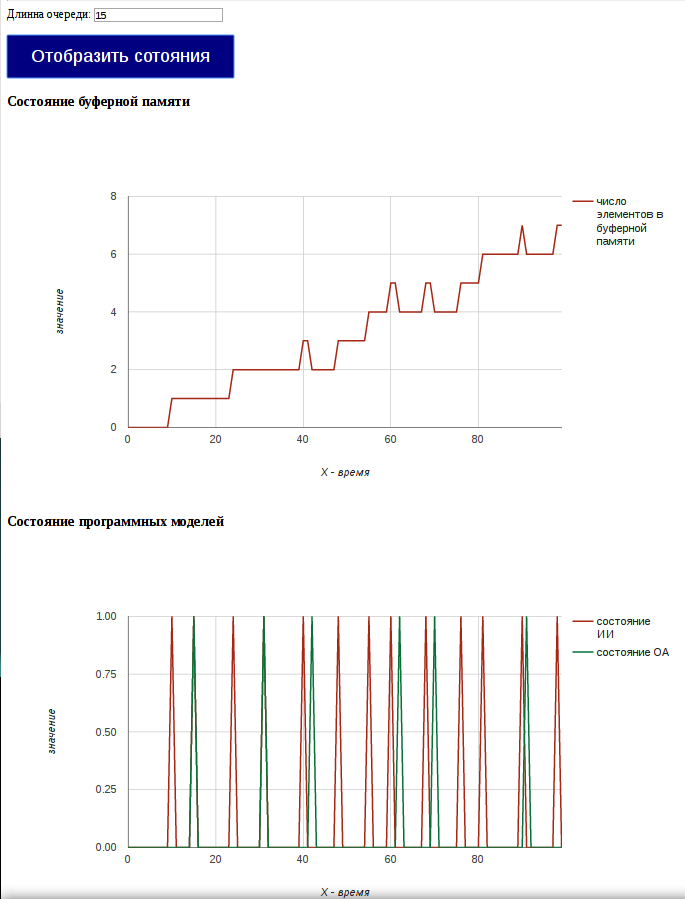
\includegraphics[scale=0.8]{screen2.png}
  \caption{Принцип $\Delta t$: графики}
\end{figure}

\begin{figure}
  \centering
  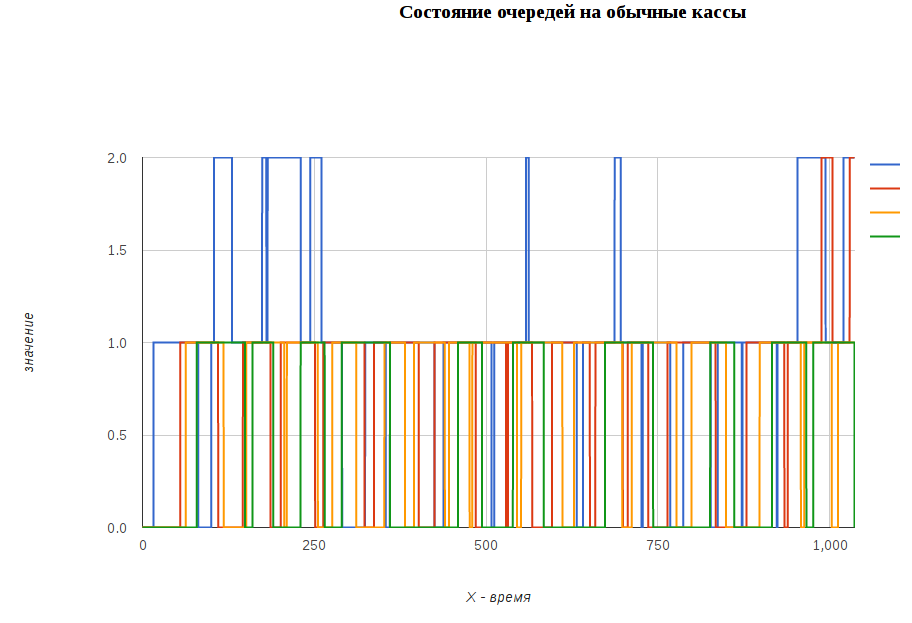
\includegraphics[scale=0.5]{screen3.png}
  \caption{Принцип событийный: поиск минимального размера буферной памяти}
\end{figure}

\begin{figure}
  \centering
  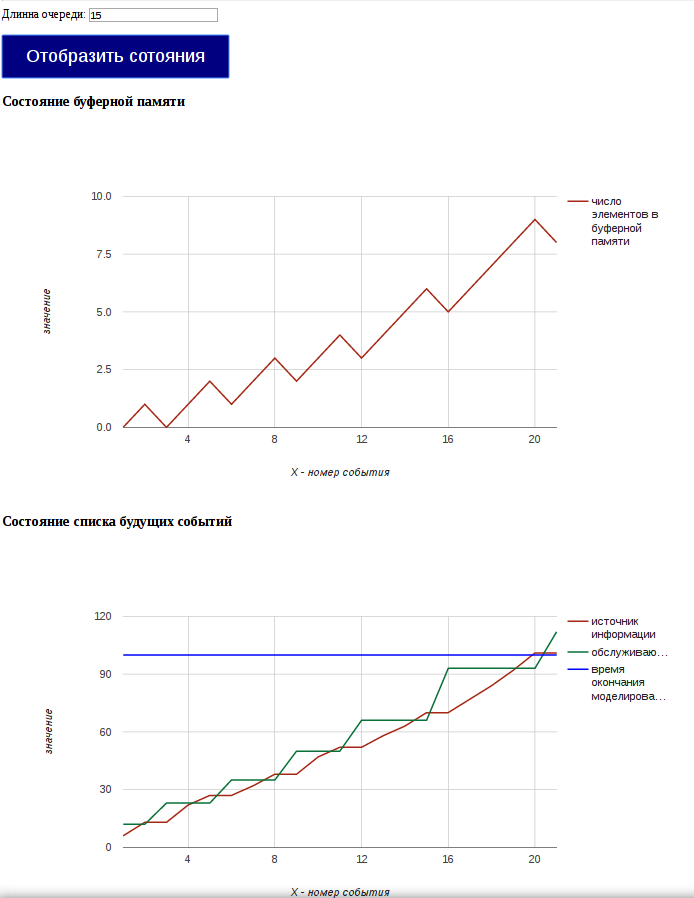
\includegraphics[scale=0.8]{screen4.png}
  \caption{Принцип событийный: графики}
\end{figure}